\subsection{Simulated rat spike data in a navigation task}

We simulated the activity of hippocampal neurons during a navigation task in a virtual linear environment. The virtual rat moved along a 1-m linear track (Figure \ref{figure:sim_movement}), with its velocity sampled from an Ornstein–Uhlenbeck (OU) process:
$$\[
dv_t = \theta \, (\mu - v_t) \, dt + \sigma \, dW_t
\]
$$
with the following parameters: $\theta$ = 1.0 (mean reversion), $\mu$ = 0.0 (long-run mean velocity, m/s), $\sigma$ = 0.4 (volatility), $v_0$=0.0 (initial velocity). The full simulation lasted 10 minutes (600 s) at a temporal resolution of 100 Hz.

\begin{figure}
    \centering
    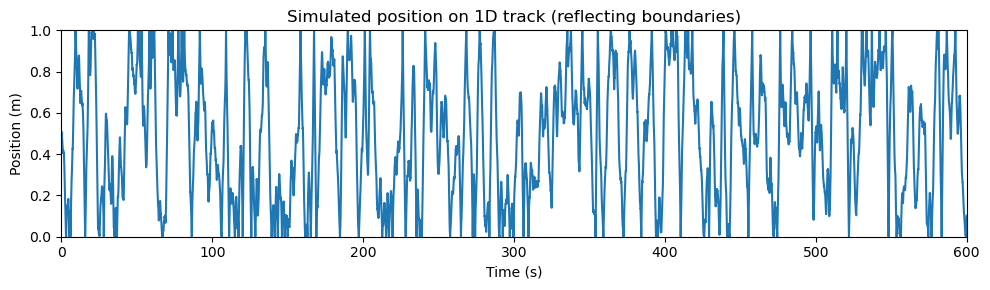
\includegraphics[width=0.9\linewidth]{paper/figures/simulated_movement.png}
    \caption{Simulated movement along the track with the Ornstein-Uhlenbeck formula. The simulated rat sampled all the positions along the track multiple times over 600 seconds. }
    \label{figure:sim_movement}
\end{figure}

We modeled four place cells along the track. Two cells had relatively broad place fields (Gaussian width $\sigma$ = 20 cm), while the other two had narrower place fields ($\sigma$ = 10 cm). This heterogeneity was intended to approximate recordings from different hippocampal subregions along the dorsoventral axis. Place fields were modeled as Gaussian functions of position with equal firing probability regardless of running direction.

The two broad fields were centered at 200 cm and 800 cm, while the two narrower fields were embedded within them at 300 cm and 900 cm, respectively. Baseline firing rates were fixed at 0.1 Hz, and peak firing rates were set to 20 Hz, 16 Hz, 18 Hz, and 15 Hz from left to right along the track (0–1000 cm) (Figure \ref{figure:ratemap_placeCells} ). 

\begin{figure}
    \centering
    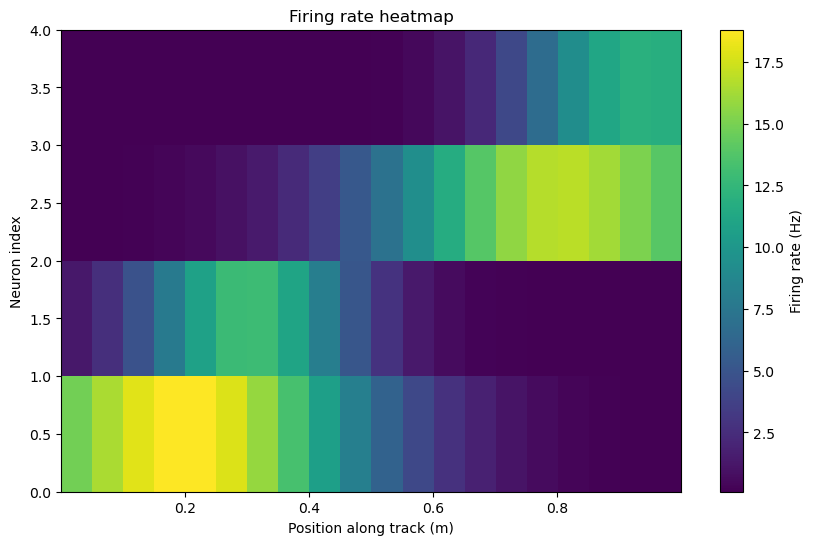
\includegraphics[width=0.75\linewidth]{paper/figures/place_cells_ratemap.png}
    \caption{Ratemap of 4 simulated place cells in a 1-meter linear track. Their place field cover the whole length of the track. }
    \label{figure:ratemap_placeCells}
\end{figure}

To mimic a larger hippocampal population, we also simulated 96 “noise” neurons whose activity was independent of position. Their mean firing rates were sampled uniformly between 1 and 5 Hz and held constant across the entire recording. Spiking activity was generated as Bernoulli draws with rate × timestep probability (figure \ref{figure:ratemap_noise}). 

\begin{figure}
    \centering
    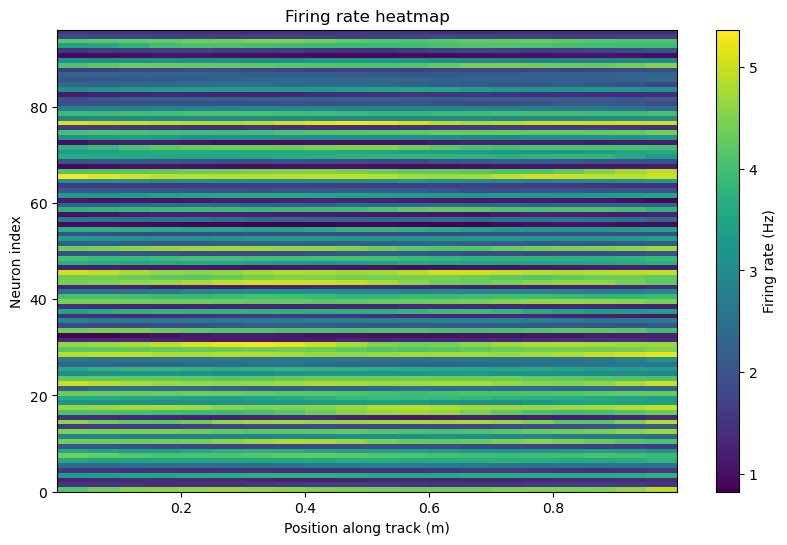
\includegraphics[width=0.75\linewidth]{paper/figures/noise_ratemap.png}
    \caption{Simulated noise along the track, the neurons had a firing rate between 1 and 5 Hz, and their firing was independent of position.}
    \label{figure:ratemap_noise}
\end{figure}

We extracted the spike count matrix from the simulation, with dimensions \textit{time samples × neurons}, and used it to train a Matryoshka Sparse Autoencoder (SAE). The model was trained with the following hyperparameters: dsae\_topk\_map=\{64:1, 128:2, 256:4\}, dsae\_loss\_x\_map=\{64:1.0, 128:1.25, 256:1.5\}.

The SAE successfully discovered a range of latent features. As expected, several features primarily reflected activity from the noise neurons, capturing random fluctuations without spatial structure. Crucially, however, a substantial subset of latent features encoded position along the track.

Two main types of spatial representations emerged:
\begin{enumerate}
    \item \textbf{Global position features}: latents whose activation varied gradually along the track, suggesting a coarse encoding of absolute position.
    \item \textbf{Local position features}: latents that exhibited sharp peaks at specific locations, resembling place-cell-like activity and corresponding to localized representations of position.
\end{enumerate}

These results demonstrate that the Matryoshka SAE can disentangle structured spatial representations from unstructured noise, recovering both global and local spatial codes (see Fig. X).

\begin{figure}
    \centering
    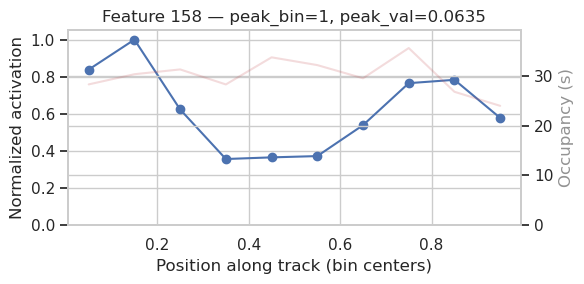
\includegraphics[width=0.5\linewidth]{paper/figures/global_position_latent_1.png}
    \caption{Enter Caption}
    \label{fig:placeholder}
\end{figure}

\begin{figure}
    \centering
    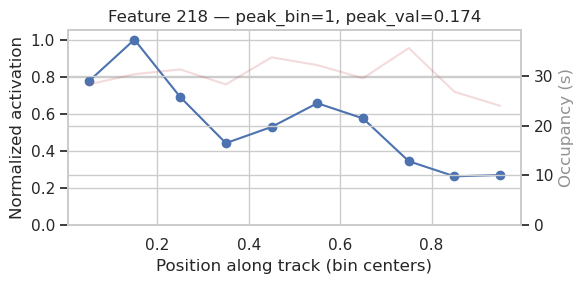
\includegraphics[width=0.5\linewidth]{paper/figures/global_position_latent_2.png}
    \caption{Enter Caption}
    \label{fig:placeholder}
\end{figure}